% ==========================================================
% Document setup
% ==========================================================
\documentclass{article}
\usepackage[margin=1.5cm, top=1cm]{geometry}

% ==========================================================
% Imported packages
% ==========================================================
\usepackage{graphicx}   % Figures
\usepackage{subcaption} % Subfigures
\usepackage{booktabs}   % Nice tables

% ==========================================================
% Title
% ==========================================================
\title{SCGSR Mid-award Progress Report Additional Materials}
\author{Jacob Hauck}
\date{June 3, 2026}

% ==========================================================
% Document
% ==========================================================
\begin{document}

\maketitle
	
% ==========================================================
% Figure 1
% ==========================================================
\begin{figure}[htb!]
	\centering
	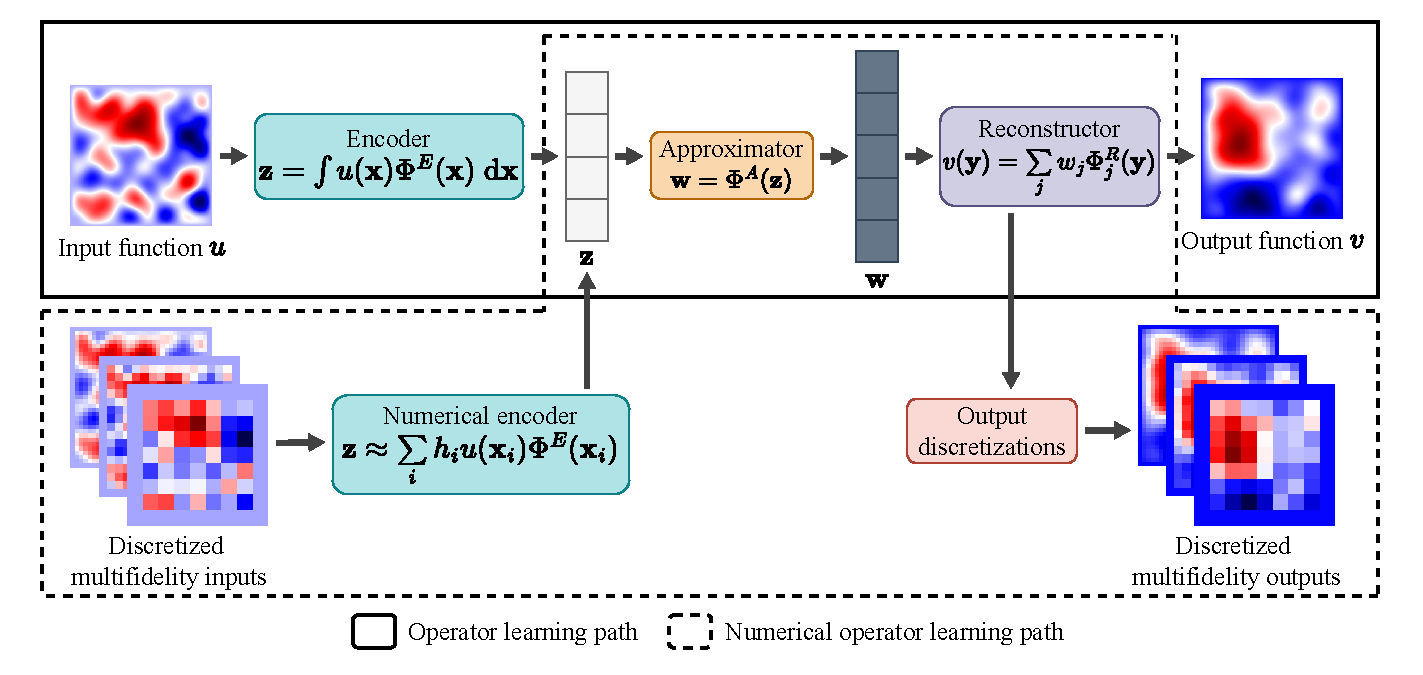
\includegraphics[width=\linewidth]{operator_learning_diagram.pdf}
	\caption{The architecture of our operator learning method, and how operator learning enables discretization independence through numerical operator learning. Note the three-module structure: (linear) encoder projects the input function onto a finite-dimensional space parameterized by neural network basis functions ($\Phi^E$), approximator approximates the operator in the latent space, and (linear) reconstructor builds the output function by taking a linear combination of neural network basis functions (using a different neural network $\Phi^R$) using the latent output variables from the approximator as weights.}
\end{figure}


% ==========================================================
% Figure 2
% ==========================================================
\begin{figure}[htb!]
	\centering
	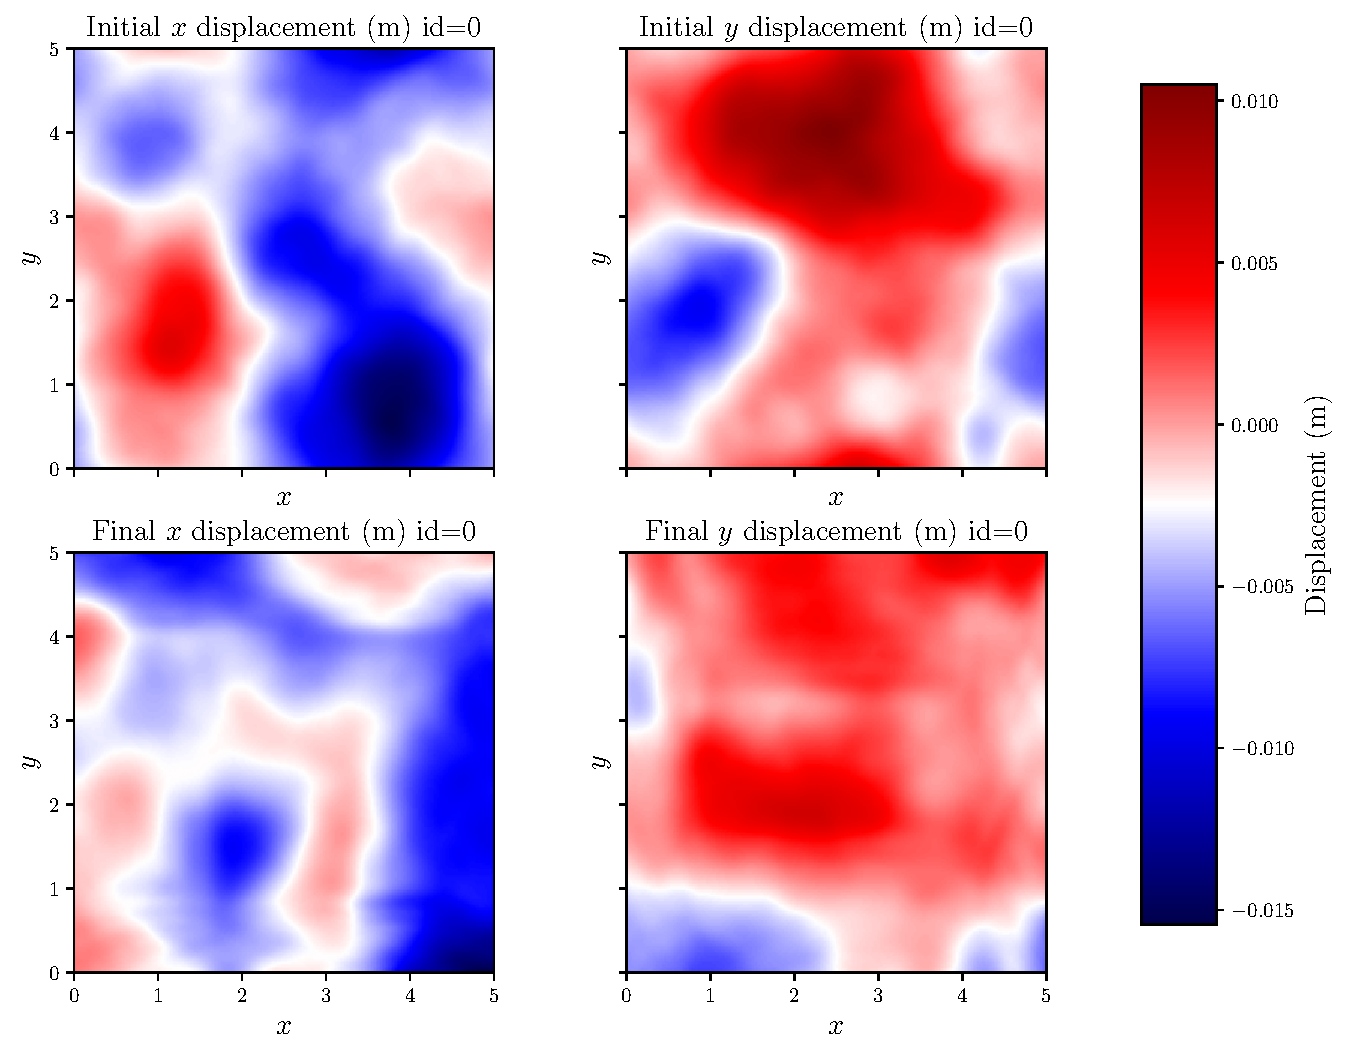
\includegraphics[width=0.8\linewidth]{example_wave_data.pdf}
	\caption{Example input--output pair from one of the wave propagation benchmark datasets, prepared using \texttt{PDMATLAB2D}. The input function is the top row, which shows the initial $x$ and $y$ displacement fields. The output function is the bottom row, which shows the final $x$ and $y$ displacement fields after a time $T = 1.8$ seconds has elapsed in the simulation. The ``id=0'' refers to this sample's ID in the dataset.}
\end{figure}


% ==========================================================
% Table 1
% ==========================================================
\begin{table}[htb!]
	\centering
	\begin{tabular}{@{}lrr@{}}
		\toprule
		Approximator & Error on training data & Error on testing data \\ 
		\midrule
		Base (3 layers, 128 neurons/layer, ReLU) & 15.2 & 18.1 \\ 
		Wide (3 layers, 384 neurons/layer, ReLU) & 12.4 & 20.7 \\
		Deep (8 layers, 128 neurons/layer, SELU) & 11.9 & 16.9 \\
		\bottomrule
	\end{tabular}
	\caption{Error (measured in \% relative $L^2$) for different approximator network settings. Using a wide approximator leads to overfitting (note gap between train and test error in the second row), but using a deep approximator with self-normalizing activation leads to a slight performance boost (compare error in first and third rows).}
\end{table}

% ==========================================================
% Figure 3
% ==========================================================
\begin{figure}[htb!]
	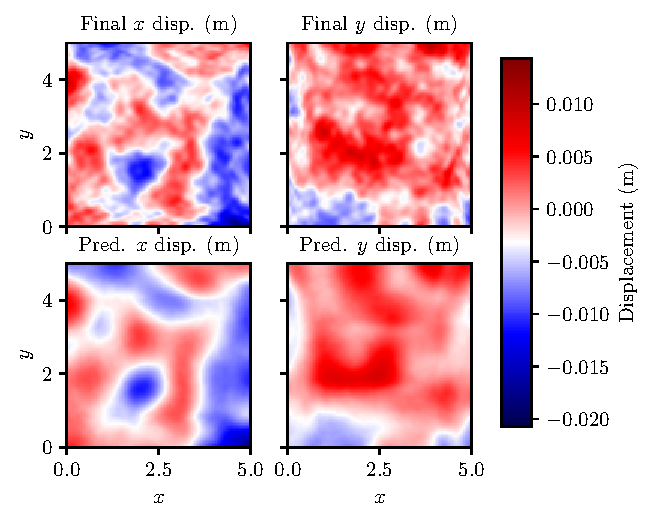
\includegraphics[width=0.33\linewidth]{test17_tg.ol.h5_pred_0.pdf}
	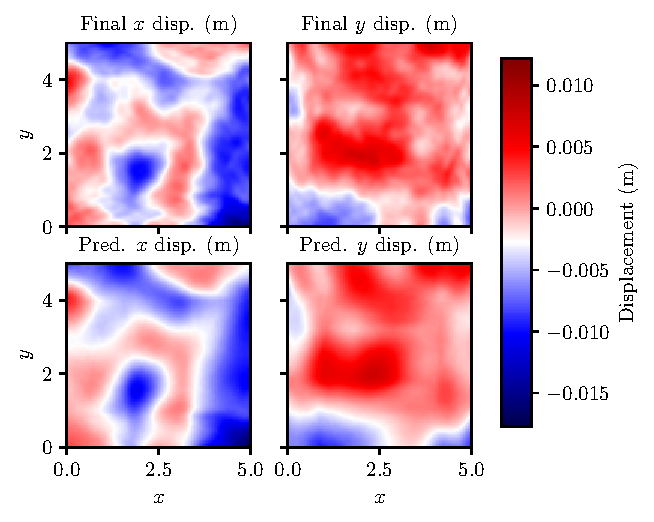
\includegraphics[width=0.33\linewidth]{test19_tg.ol.h5_pred_0.pdf}
	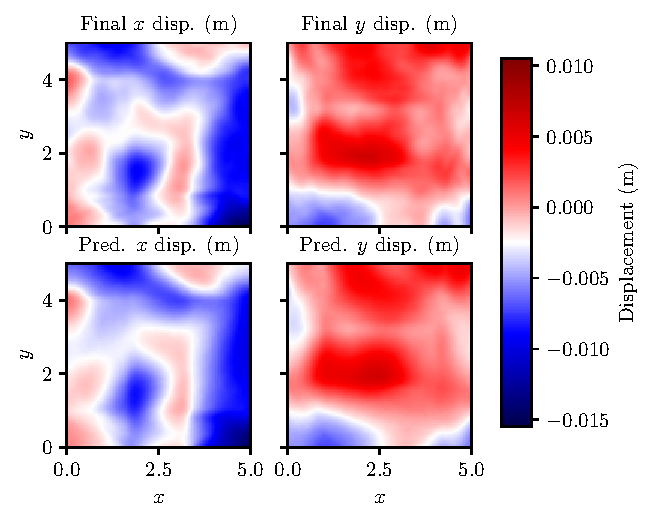
\includegraphics[width=0.33\linewidth]{test21_tg.ol.h5_pred_0.pdf}
	\caption{Example final displacement fields (top row, $x$ and $y$ components alternating) and corresponding model predictions (bottom row) for different input Gaussian process covariance eigenvalue decay rates. Decay rate increases from left to right. Note the corresponding decrease in strong high-frequency components from left to right. Also note how the model prediction only capture low-frequency (smooth) components, making its predictions more accurate when the covariance eigenvalues decay quickly.}
\end{figure}

% ==========================================================
% Figure 4
% ==========================================================
\begin{figure}[htb!]
	\centering
	\begin{subfigure}[t]{0.49\linewidth}
		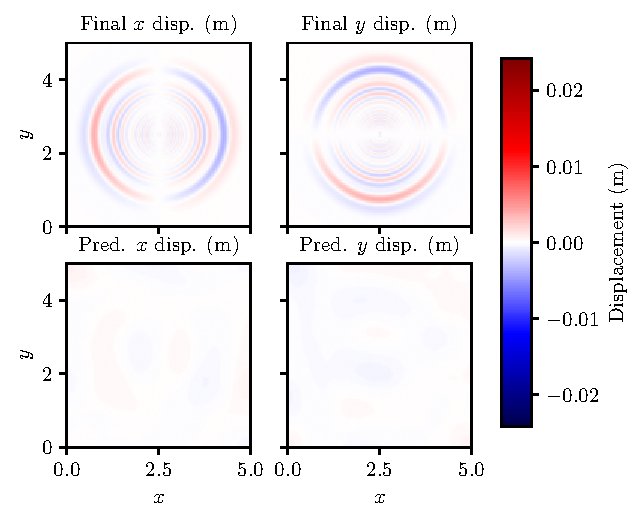
\includegraphics[width=\linewidth]{BumpProp1.ol.h5_pred_0.pdf}
		\subcaption{Initial displacement scale = $0.03$}
	\end{subfigure}
	~
	\begin{subfigure}[t]{0.49\linewidth}
		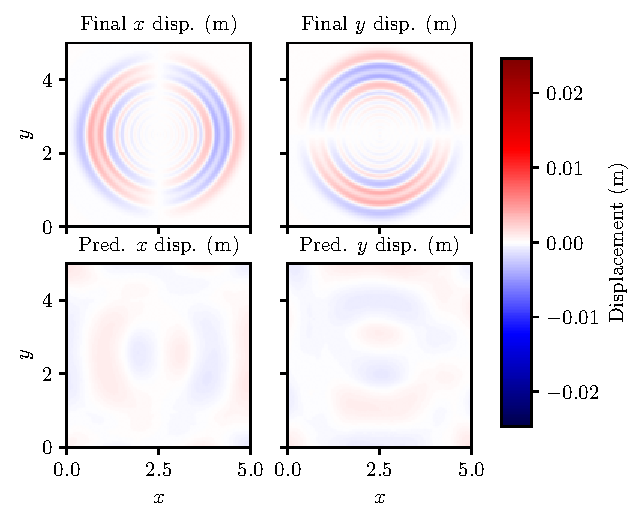
\includegraphics[width=\linewidth]{BumpProp5.ol.h5_pred_0.pdf}
		\subcaption{Initial displacement scale = $0.05$}
	\end{subfigure}
	~
	\begin{subfigure}[t]{0.49\linewidth}
		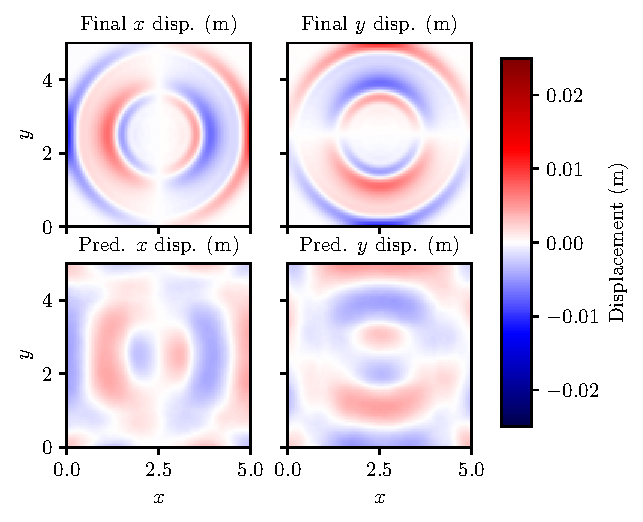
\includegraphics[width=\linewidth]{BumpProp4.ol.h5_pred_0.pdf}
		\subcaption{Initial displacement scale = $0.10$}
	\end{subfigure}
	~
	\begin{subfigure}[t]{0.49\linewidth}
		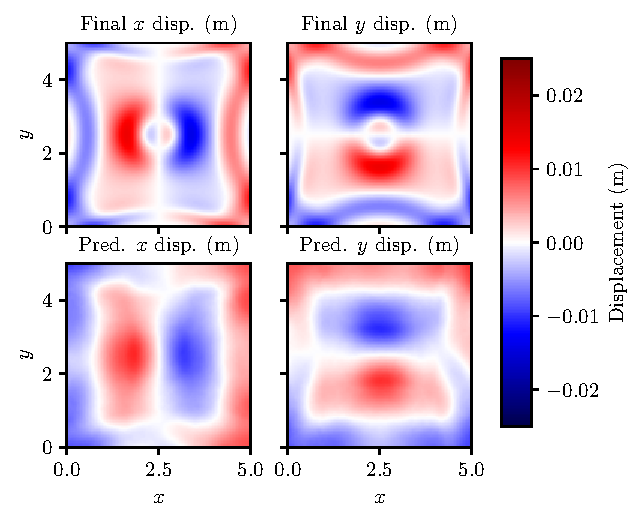
\includegraphics[width=\linewidth]{BumpProp3.ol.h5_pred_0.pdf}
		\subcaption{Initial displacement scale = $0.20$}
	\end{subfigure}
	~
	\begin{subfigure}[t]{0.5\linewidth}
		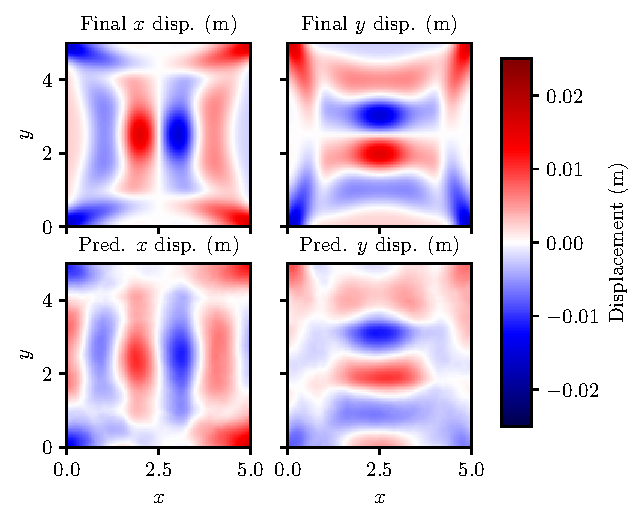
\includegraphics[width=\linewidth]{BumpProp2.ol.h5_pred_0.pdf}
		\subcaption{Initial displacement scale = $0.30$}
	\end{subfigure}
	\caption{Model predictions for out-of-distribution test initial displacements. The top row in each block shows simulation final displacement field $x$ and $y$ components, and the bottom rows show the corresponding model predictions. Input initial displacement fields are Gaussian bumps of varying sizes, specified in the captions of each subfigure. The model makes more accurate predictions for larger bumps (which have less high-frequency information and result in less dispersive effects).}
\end{figure}

% ==========================================================
% Table 2
% ==========================================================
\begin{table}[htb!]
	\centering
	\begin{tabular}{@{}rrr@{}}
		\toprule
		$T$ & Error on training data & Error on testing data \\
		\midrule
		1.8 & 15.4 & 18.2 \\
		1.4 & 16.5 & 21.0 \\
		1.0 & 16.0 & 19.3 \\
		0.6 & 14.1 & 17.1 \\
		0.2 & 14.4 & 19.2 \\
		\bottomrule
	\end{tabular}
	\caption{Independence of model error (measured in \% relative $L^2$) on simulation duration $T$. When $T = 0.2$, the operator is nearly the identity, suggesting that the reconstructor module in our model is insufficient. Addressing this limitation will be the focus of the remaining work on the wave propagation problem.}
\end{table}

% ==========================================================
% Figure 5
% ==========================================================
\begin{figure}[htb!]
	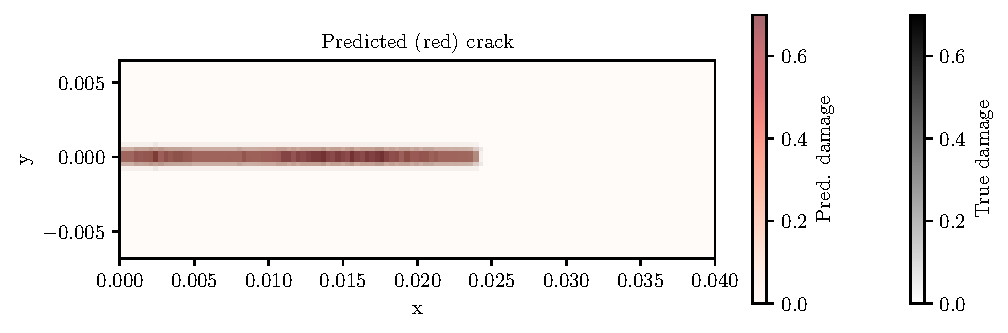
\includegraphics[width=\linewidth]{compare_200.pdf}
	\caption{An example crack final damage field (black) and model prediction superimposed (red) in the case of symmetric traction on the top and bottom of the plate. This image is cropped to show only the part of the crack that grew. Note that the damage field refers to the fraction of broken bonds (between 0 and 1) per particle. The model prediction agrees closely with the true crack path.}
\end{figure}


% ==========================================================
% Figure 6
% ==========================================================
\begin{figure}[htb!]
	\begin{subfigure}[t]{0.33\linewidth}
		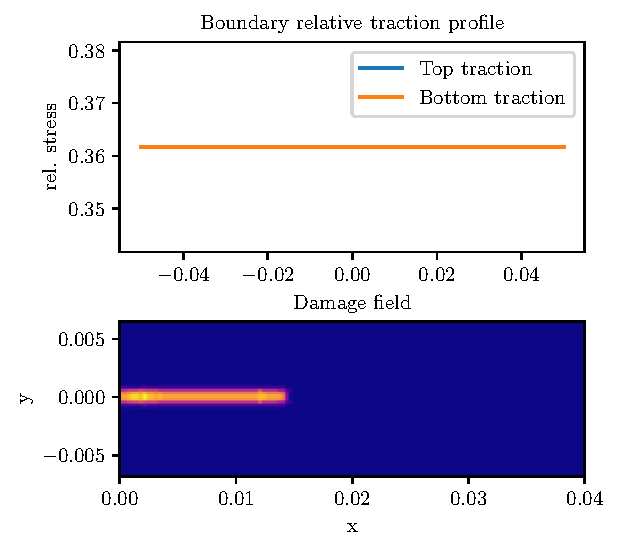
\includegraphics[width=\linewidth]{sym_uniform_290.pdf}
		\subcaption{Symmetric, uniform traction}
	\end{subfigure}
	~
	\begin{subfigure}[t]{0.33\linewidth}
		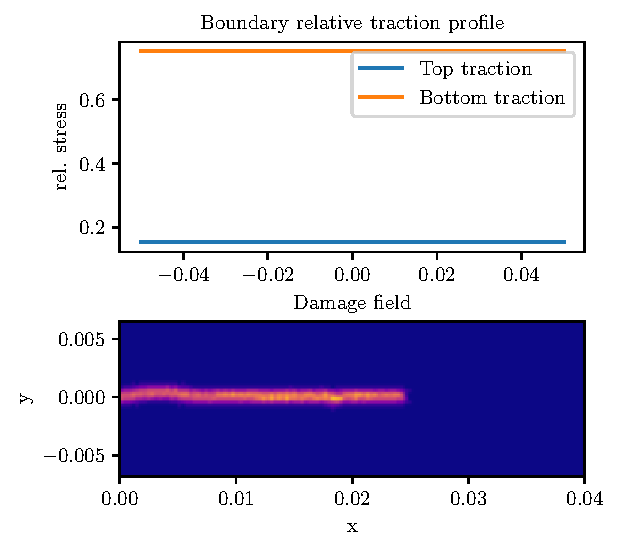
\includegraphics[width=\linewidth]{asym_uniform_65.pdf}
		\subcaption{Asymmetric, uniform traction}
	\end{subfigure}
	~
	\begin{subfigure}[t]{0.33\linewidth}
		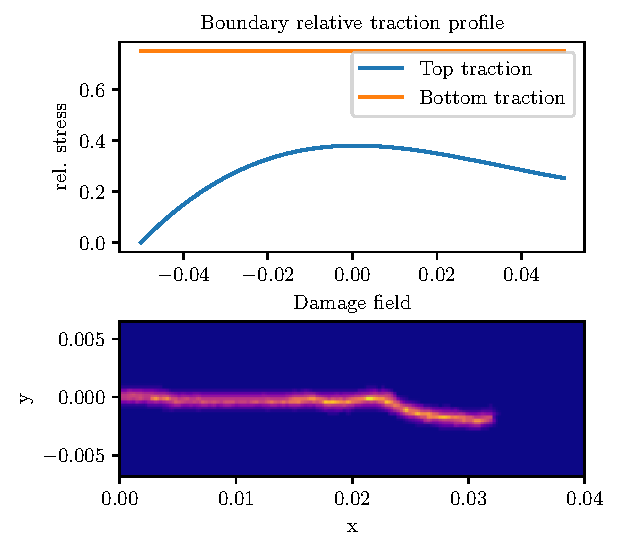
\includegraphics[width=\linewidth]{asym_nonuniform_324.pdf}
		\subcaption{Asymmetric, uniform traction}
	\end{subfigure}
	\caption{Samples from generated crack propagation datasets. The input function is the boundary relative traction profile (top row, units are relative to a fixed, maximum traction), and the output function is the final damage field (bottom row, cropped to the region around where the crack grew). Note that dark blue means no damage, and orange/white means high damage. The goal for operator learning on these datasets is to predict the final crack path.}
\end{figure}


% ==========================================================
% Figure 7
% ==========================================================
\begin{figure}[htb!]
	\begin{subfigure}[t]{0.49\linewidth}
		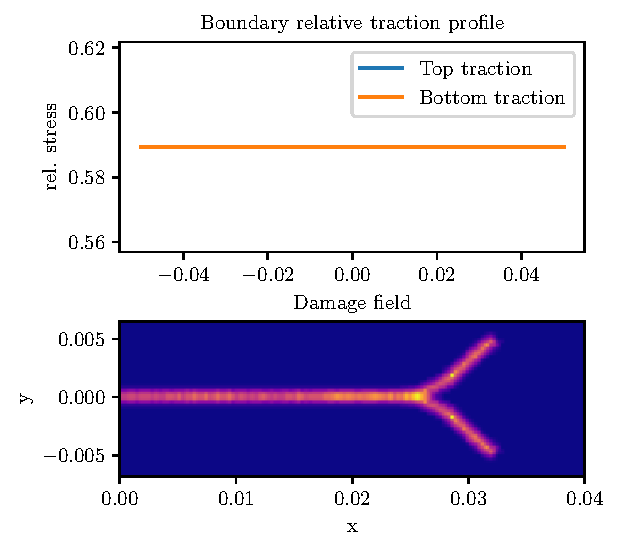
\includegraphics[width=\linewidth]{unstable_118.pdf}
	\end{subfigure}
	~
	\begin{subfigure}[t]{0.49\linewidth}
		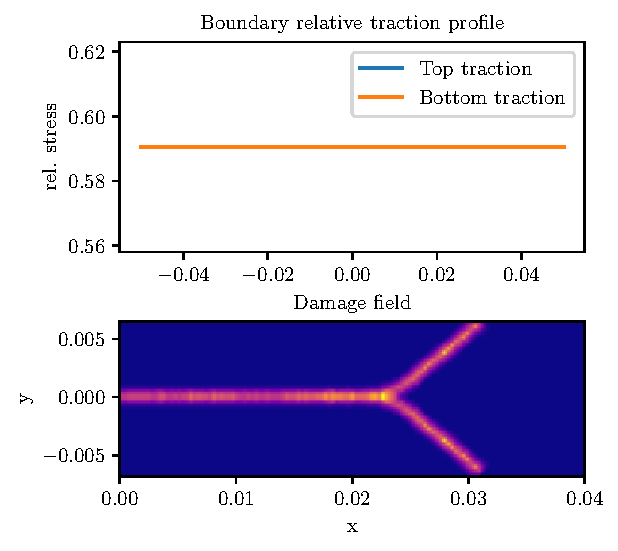
\includegraphics[width=\linewidth]{unstable_119.pdf}
	\end{subfigure}
	\caption{Comparison of simulated crack paths with symmetric, uniform relative traction that differs in strength by less than 1\%. The simulation produces very different results despite the nearly identical parameters. This makes prediction with operator learning nearly impossible, so finding a stable configuration is a top priority for the remaining time in my award.}
\end{figure}


% ==========================================================
% Figure 8
% ==========================================================
\begin{figure}[htb!]
	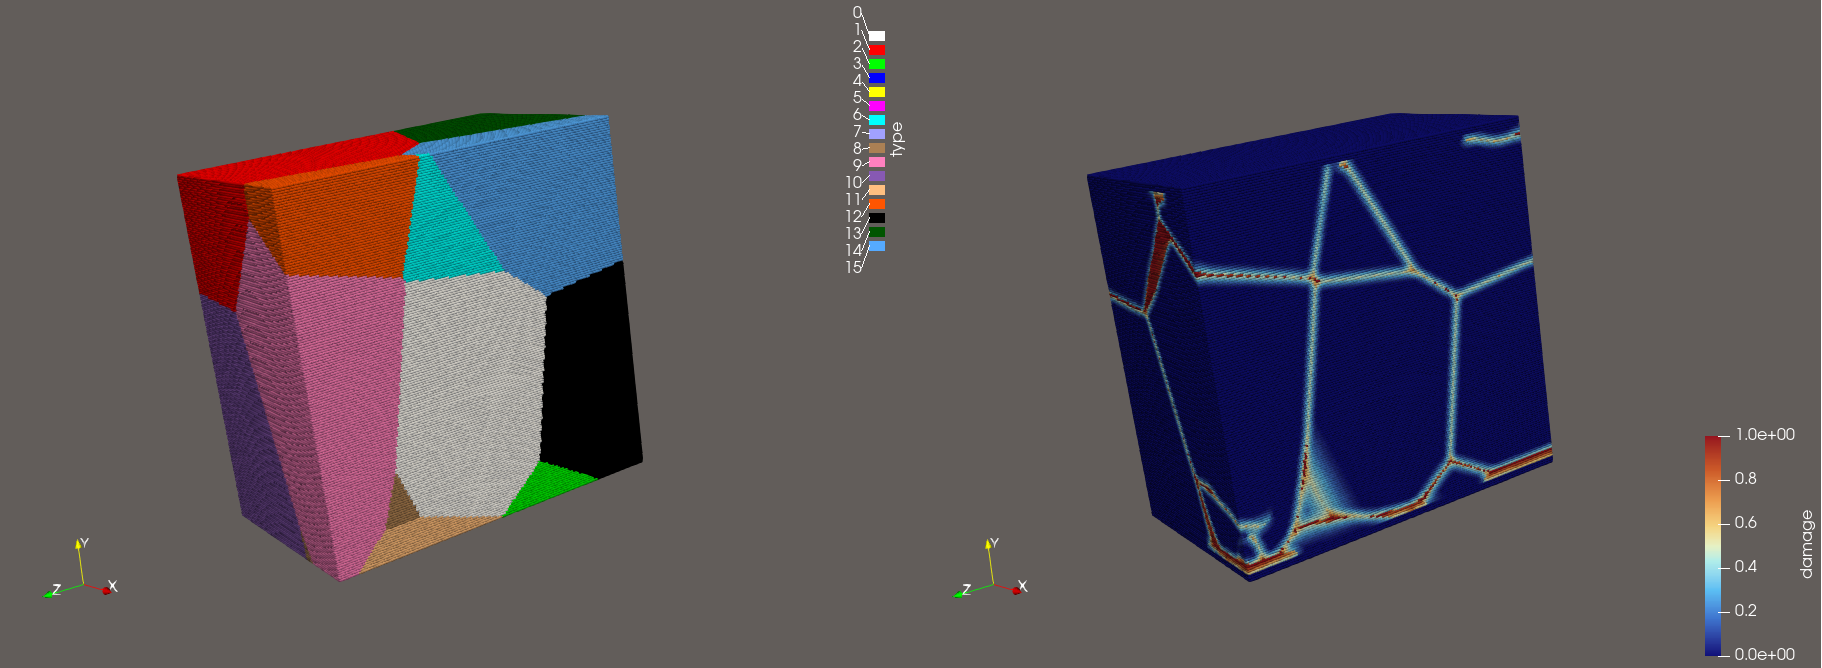
\includegraphics[width=\linewidth]{polycrystal_damage_cube.png}
	\caption{Grain structure (left) and final damage field (right) in a small, cube-shaped polycrystal with 16 grains. Simulation was performed with CabanaPD. This view shows a cross-section of the cube perpendicular to the $x$ axis.}
\end{figure}


\end{document}
